\chapter{Variedades}\label{cap_var}

\thispagestyle{empty}

Este capítulo apresenta definições sobre variedades, variedades lineares por partes. Ele também cita alguns teoremas da literatura que são importantes para que os algoritmos apresentados neste livro funcionem corretamente. 
As definições e teoremas apresentados neste capítulo são de grande importância para a leitura do restante do texto, pois os conceitos serão utilizados nos capítulos que tratam de aproximações lineares por partes de variedades definidas implicitamente, que é o foco deste livro.
As provas dos teoremas citados não serão apresentadas, porém referências para tais provas se encontram ao longo do texto.
As definições e teoremas das primeiras seções serão utilizadas nas demais seções deste capítulo e dos capítulos seguintes.

%Este capítulo é matematicamente denso. Caso o leitor esteja interessado primordialmente na parte prática dos algoritmos, e tenha alguma familiaridade com topologia, geometria e interpolação de funções, sugerimos começar pelo o Capítulo~\ref{cap_cont_enum} e usar este aqui como referência. 

\markboth{Variedades}{Variedades Diferenciáveis}
\section{Variedades Diferenciáveis}\label{var_dif}

Vamos apresentar alguns conceitos básicos sobre variedades diferenciáveis, mais especificamente variedades definidas implicitamente. 
Para detalhes e provas sugerimos a leitura dos livros clássicos  ``Curso de Análise Vol. 2" \cite{elon_an} e ``Variedades Diferenciáveis" de Elon Lages Lima \cite{elon}, em ``Introdução aos Sistemas Dinâmicos" de Jacob Palis Junior  e Welington de Melo \cite{jacob} e em ``Toplology form the Differentiable Viewpoint"  de John Milnor \cite{Mi}.

\begin{defi} $($Homeomorfismo$)$
Uma aplicação $f : U \rightarrow V$ é um homeomorfismo se é uma aplicação contínua, invertível e sua inversa $f^{-1} : V \rightarrow U$ é uma aplicação contínua.
Neste caso dizemos que $U$ e $V$ são homeomorfos.
\end{defi}

\begin{defi} $($Difeomorfismo$)$
Uma aplicação $f : U \rightarrow V$ é um difeomorfismo de classe $C^r$ $(1 \le r \le \infty)$ se é uma aplicação invertível e sua inversa $f^{-1} : V \rightarrow U$ é uma aplicação de classe $C^r$.
Neste caso dizemos que $U$ e $V$ são difeomorfos.
\end{defi}

\begin{defi} $($Valor Regular$)$
Seja $f : U \subset \R^n \rightarrow \R^k$ uma aplicação de classe $C^r$ $(r \ge 1)$.  $c \in \R^k$ é valor regular de $f$ se para todo $x \in f^{-1}(c)$, $Df(x): \R^n \rightarrow \R^k$ tem posto máximo.  Se $c$ n\~ao for valor regular de $f$, diremos que \'e valor cr\'{\i}tico de $f$. 
\end{defi}

\begin{teore} $($Função Inversa$)$
Sejam $U \subset \R^n$ um aberto e $f : U \rightarrow \R^n$ uma aplicação de classe $C^r$ $(1 \le r \le \infty)$ tal que, em um ponto $x_0 \in U$, a derivada $Df(x_0)$ é um isomorfismo. Então $f$ aplica difeomorficamente uma vizinhança menor $V$ de $x_0$ sobre uma vizinhança $W$ de $f(x_0)$.
\end{teore}

\begin{teore} $($Função Implícita$)$
Sejam $U \subset \R^m \times \R^n$ um aberto e $f : U \rightarrow \R^n$ uma aplicação de classe $C^r$ $(1 \le r \le \infty)$. Sejam  $z_0 = (x_0,y_0) \in U$ e $c = f(z_0)$. 
Suponha que a derivada em relação a segunda variável $D_2f(z_0): \R^n \rightarrow \R^n$ seja um isomorfismo. 
Então existem abertos $V \subset \R^m$ contendo $x_0$, e $W \subset U$ contendo $z_0$, tais que, para cada $x \in V$, existe um único $\xi(x) \in \R^n$, com $(x,\xi(x)) \in W$ e $f(x,\xi(x)) = c$.
A aplicação $\xi : V \rightarrow \R^n$, assim definida, é de classe $C^r$ e sua derivada é dada por
$D\xi(x) = [D_2f(x,\xi(x))]^{-1} \cdot D_1f(x,\xi(x))$.
\end{teore}

\begin{defi} $($Variedade Diferenciável$)$
$\mathcal{M} \subset \R^m$ é uma variedade diferenciável de dimensão $n$ e de classe $C^r$ $(1 \le r \le \infty)$ 
se para todo $x \in \mathcal{M}$ existirem vizinhanças abertas $U \subset \R^m$ de $x$, 
$V \subset \R^{n-1} \times \R^{+}$ e um difeomorfismo de classe $C^r$ de $\mathcal{M} \cap U$ em $V$.  
Um difeomorfismo $\varphi : U \cap \mathcal{M}  \rightarrow V$ \'e chamado de parametriza\c c\~ao da regi\~ao $U \cap \mathcal{M}$. A fronteira de $\mathcal{M}$, $\partial \mathcal{M}$ \'e o conjunto dos pontos de $\mathcal{M}$ correspondentes a $\R^{n-1} \times \{0\}$ pelas parametriza\c c\~oes. 
\end{defi}

\begin{figure}[h]
\begin{center} 
\includegraphics*[angle=0,scale=0.5]{imagens/cap2/BoysSurfaceTopView.eps} 
\caption{Proje\c{c}\~ao em $\R^3$ do plano projetivo. Figura extraída de \url{https://commons.wikimedia.org/wiki/File:BoysSurfaceTopView.eps} } 
\label{fig.BoySurface}
\end{center}
\end{figure}


\begin{figure}[h]
\begin{center} 
\includegraphics*[angle=0,scale=0.5]{imagens/cap2/KleinBottle-01.eps} 
\caption{Superfície não orientável chamada de {\bf garrafa de Klein}. Figura extraída de \url{https://commons.wikimedia.org/wiki/File:KleinBottle-01.eps} } 
\label{fig.BoySurface}
\end{center}
\end{figure}

\begin{defi} $($Espaço Tangente$)$
Sejam $\mathcal{M}$ uma variedade diferenci\'avel de dimens\~ao $n$ e $\varphi : V \rightarrow U \cap \mathcal{M}$ uma parametriza\c c\~ao de $U \cap \mathcal{M}$, onde $\varphi(u) = v$.
Definimos o espa\c co vetorial tangente a $\mathcal{M}$ no ponto $v$ como $T_{v}\mathcal{M} = \{ D\varphi(u) \cdot y \; | \; y \in {\R}^{n}\}$, onde $D\varphi(u)$ é o operador derivada da parametrização $\varphi$ no ponto $u \in V$. 
\end{defi}

\begin{teore} $($Variedade Definida Implicitamente$)$ \label{teo_VI}
Sejam $U \subset \R^n$ um aberto e $f : U \rightarrow \R^k$ uma aplicação de classe $C^r$ $(1 \le r \le \infty)$.
Se $c \in \R^k$ é valor regular de $f$, ou $f^{-1}(c)$ é vazio ou é uma variedade diferenciável de dimensão $n-k$ e de classe $C^r$ em $\R^n$.
Além disso, para todo $p \in f^{-1}(c)$, o espaço tangente em $p$ é o núcleo de $Df(p): \R^n \rightarrow \R^k$.
\end{teore} 

\begin{teore} $($Vizinhança Tubular$)$ \label{teo_VT}
Seja $F : U \rightarrow \R^{n}$ uma aplica\c c\~ao de classe $C^{r}$ no 
aberto $U \subset \R^{m}$ com $m \geq n$ e $1 \le r \le \infty$. 
Se $c \in  \R^{n}$ \'e um valor regular de $F$, ent\~ao existe uma vizinhan\c ca fechada $V_{\mathcal{M}}$ da variedade $\mathcal{M} = F^{-1}(c)$ constitu\'{\i}da de variedades, isto \'e, se $x \in V_{\mathcal{M}}$, ent\~ao $F^{-1}(F(x))$ \'e uma variedade contida em $V_{\mathcal{M}}$.
\end{teore} 

\begin{defi} $($Conjunto de Medida Nula$)$
Uma conjunto $X \subset \R^n$ é um conjunto de medida nula em $\R^n$ se para cada $\epsilon > 0$ dado, é possível obter uma sequência de hipercubos de dimensão $n$ abertos $C_1, C_2,\ldots,C_k,\ldots$ em $\R^n$ tais que $X \subset \cup_{k=1}^\infty C_k$ e $\sum_{k=1}^\infty vol(C_k) < \epsilon$.
\end{defi}

\begin{defi} $($Conjunto Denso$)$
Uma conjunto $X \subset \R^n$ é um conjunto denso em $\R^n$ se o complementar $R^n - X$ tem medida nula em $\R^n$.
\end{defi}

\begin{teore} $($Sard$)$ \label{Teo_Sard}
Seja $f : U \subset \R^n \rightarrow \R^k$ uma aplicação de classe $C^r$ $(r \ge max\{1,n-k+1\})$. 
O conjunto dos valores regulares de $f$ é aberto e denso em $\R^k$.
\end{teore}

\begin{defi} $($Subvariedade Diferenciável$)$
Seja $\mathcal{M} \subset \R^m$ uma variedade diferenciável de dimensão $n$ e de classe $C^r$ $(1 \le r \le \infty)$. 
$\mathcal{N} \subset \mathcal{M}$ é uma subvariedade diferenciável de dimensão $k$ de $\mathcal{M}$ e de classe $C^s$ $(1 \le s \le r)$ 
se para todo $x \in \mathcal{N}$ existirem vizinhanças abertas $U \subset \R^m$ de $x$, 
$V \subset \R^{k-1} \times \R^{+}$ e um difeomorfismo de classe $C^s$ de $\mathcal{N} \cap U$ em $V$.  
\end{defi}

\begin{defi} $($Transversalidade$)$ \label{def_TR}
Sejam $\mathcal{M}$ e $\mathcal{N}$ duas variedades de dimensão $m$ e $n$ respectivamente em $\R^k$ $(k \ge max\{m , n\})$ e de classe $C^r$ $(1 \le r \le \infty)$. 
Dizemos que $\mathcal{M}$ e $\mathcal{N}$ são transversais em um ponto $p \in \mathcal{M} \cap \mathcal{N}$ se $T\mathcal{M}_p + T\mathcal{N}_p = \R^k$.
Se $\mathcal{M} \cap \mathcal{N} = \emptyset$, ent\~ao $\mathcal{M}$ e $\mathcal{N}$ s\~ao transversais por vacuidade.
\end{defi}




\markboth{Variedades}{Variedades Lineares por Partes}
\section{Variedades Lineares por Partes}\label{cap_var_lin_par}

Para maior aprofundamento no tema apresentado nesta e nas pr\'oximas seções, \'e sugerida a leitura da tese~\cite{Cas92}, do livro~\cite{AlGe90}, do artigo~\cite{Cas06} e do curso no proceedings~\cite{Eaves76}. 

\begin{defi} $($Espaço Afim$)$
Dados os pontos $v_{0},v_{1},\ldots,v_{k} \in \R^{n}$, chama-se o conjunto 
$aff(v_{0},\ldots,v_{k}) =$ 
$\{ v \in  \R^{n} \; |$ $ \sum_{i=0}^{k} \lambda_{i} v_{i} = v$ e 
$\sum_{i=0}^{k} \lambda_{i} = 1\}$ de conjunto afim gerado pelos pontos
$v_{0},\ldots,v_{k}$.  
\end{defi}

\begin{defi} $($Dimensão$)$
Chama-se de dimens\~ao de $aff(v_{0},\ldots,v_{k})$ 
e denota-se por $dim(aff(v_{0},\ldots,v_{k}))$ o maior n\'umero de vetores 
linearmente independentes entre os do conjunto
$\{v_{1}-v_{0},\ldots,v_{k}-v_{0}\}$.
\end{defi}

\begin{defi} $($Célula Convexa Afim$)$
Chama-se de c\'elula convexa afim, gerada pelos
pontos $v_{0},v_{1},\ldots,v_{k}$, o conjunto 
$\sigma = [v_{0},\ldots,v_{k}]$ $ = \{ v \in  \R^{n} \; | \;
\sum_{i=0}^{k} \lambda_{i} v_{i} = v, \sum_{i=0}^{k} \lambda_{i} = 1$
e $\lambda_{i} \geq 0 \}$. Definimos a dimens\~ao de $\sigma$ por
$dim(\sigma) =$ $dim(aff(v_{0},\ldots,$ $v_{n}))$. 
Uma célula convexa afim $\sigma$ de dimensão $k$ é denominada $k$-célula.
\end{defi}

\begin{figure}[h]
\begin{center}
\begin{tabular}{ccc}
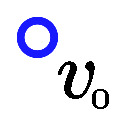
\includegraphics[angle=0,scale=0.45]{imagens/cap2/fig6-0.eps} & \hspace{0.5cm} 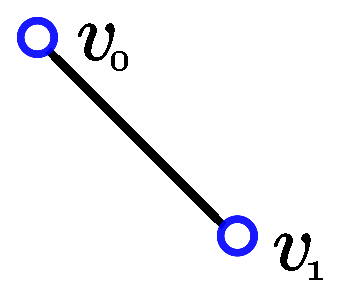
\includegraphics[angle=0,scale=0.45]{imagens/cap2/fig6-1.eps} & \hspace{0.5cm}
 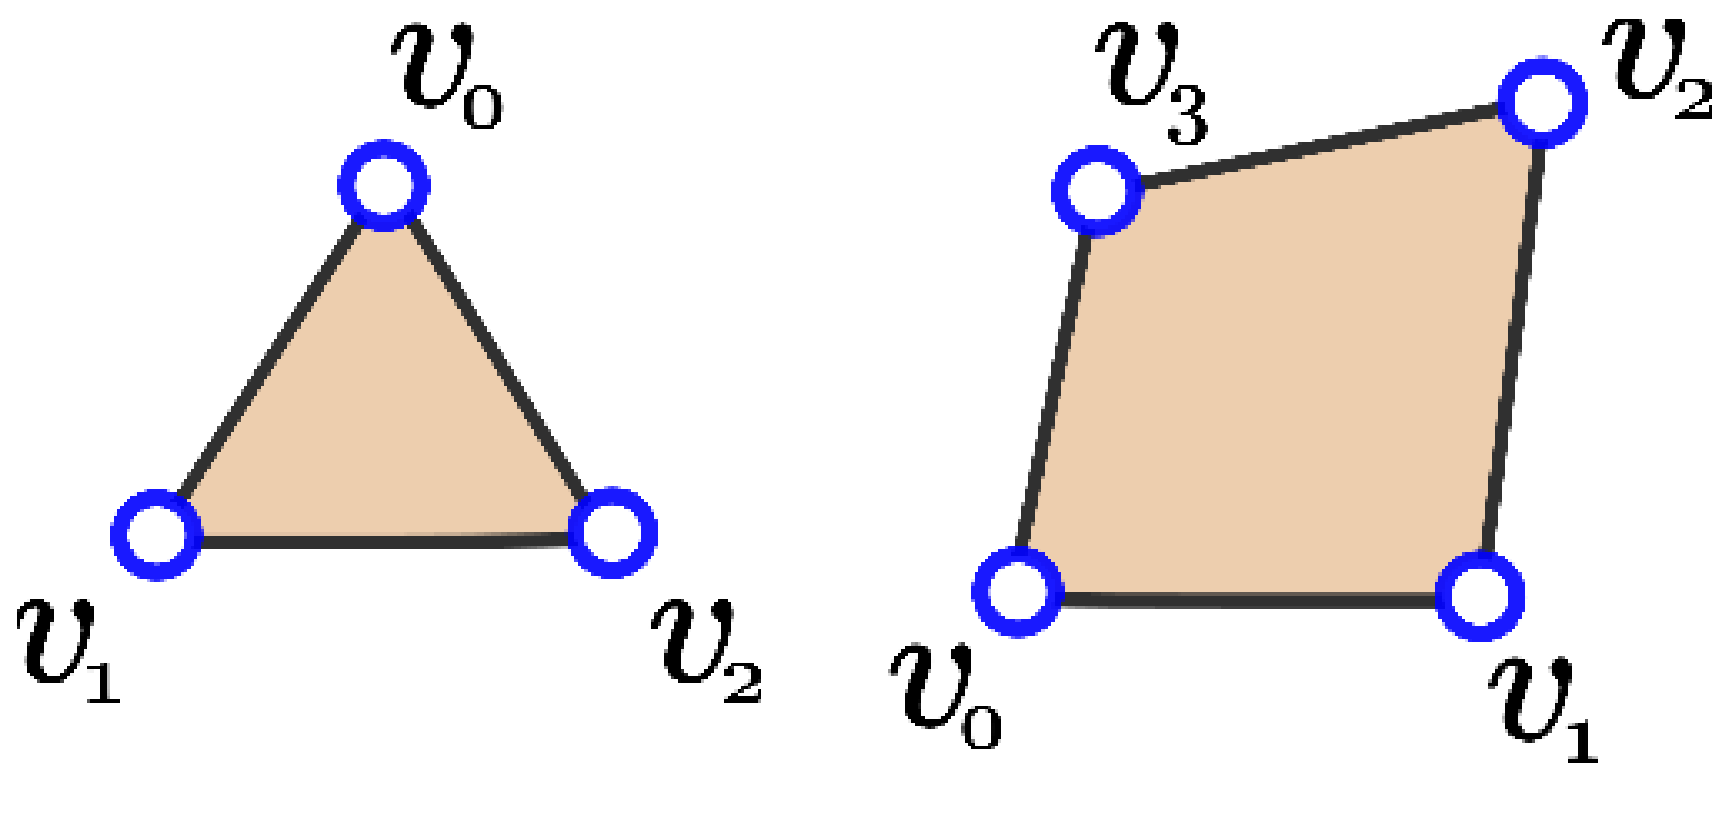
\includegraphics[angle=0,scale=0.2]{imagens/cap2/fig6-2.eps}\\
 0-célula & \hspace{0.5cm} 1-célula & \hspace{0.5cm} 2-célula\\
 \end{tabular} 
 \begin{tabular}{c}
 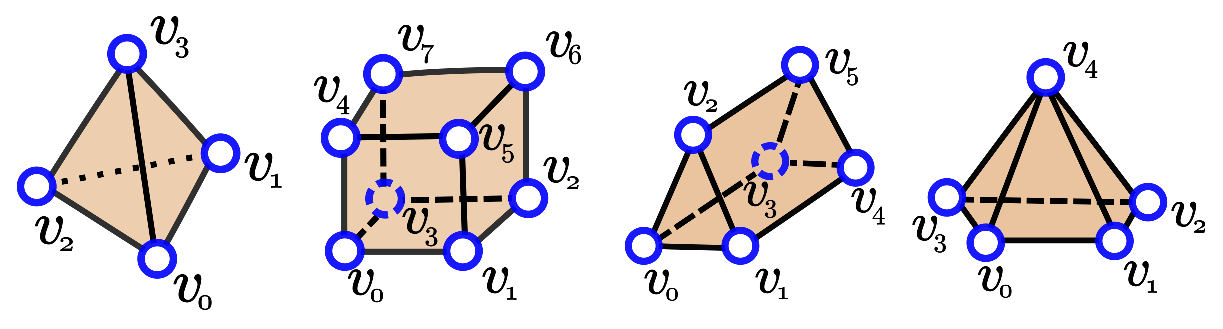
\includegraphics[angle=0,scale=0.65]{imagens/cap2/fig6-3.eps} \\
3-célula \\
\end{tabular}
\end{center}
\caption{Exemplos de 0-célula, 1-célula, 2-células e 3-células.}
\end{figure}


\begin{defi} $($Bordo de uma Célula Convexa Afim$)$
O bordo de uma c\'elula convexa afim $\sigma$, denotada por $\partial(\sigma)$,
é o conjunto de sub-células satisfazendo:
\begin{enumerate}
\item Se $\sigma' \in \partial(\sigma)$, então $\sigma'$ é gerada por um subconjunto de vértices de $\sigma$;
\item Para qualquer $p \in \sigma' \in \partial(\sigma)$, não existe uma bola contendo $p$ em $aff(\sigma)$ inteiramente contida em $\sigma'$;
\item Se $\sigma'_1, \sigma'_2 \in \partial(\sigma)$ e tem a mesma dimensão então  $\sigma'_1 \nsubseteq \sigma'_2$ e $\sigma'_2 \nsubseteq \sigma'_1$.
\end{enumerate}
\end{defi}

\begin{defi} $($Face de uma Célula Convexa Afim$)$
Sejam uma célula convexa afim $\sigma = [v_{0},\ldots,v_{m}]$ de dimensão $n$ e
$\tau = [\omega_{0},\ldots,\omega_{l}]$ uma célula convexa afim de dimensão $k$,
com $\{\omega_{0},\ldots,\omega_{l}\} \subset \{v_{0},\ldots,v_{m}\}$, 
então $\tau$ é uma face de $\sigma$ se:
\begin{enumerate}
\item $\tau \subset \partial(\sigma)$; 
\item Se existe alguma sub-célula $\eta$ com $aff(\tau) = aff(\eta)$, então $\eta \subset \tau$.
\end{enumerate}
\end{defi}

\begin{defi} $($Decomposição Celular$)$
Uma cole\c c\~ao $\mathcal{C}$ de c\'elulas convexas afins 
\'e dita decomposi\c c\~ao celular de um conjunto $S \subset  \R^{n}$ se:
\begin{enumerate}
\item $S = \bigcup_{\sigma \in \mathcal{C}}\ \sigma$;
\item Se $\sigma_{1},\sigma_{2} \in \mathcal{C}$, ent\~ao $\sigma_{1} \cap \sigma_{2} = 
         \emptyset$ ou $\sigma_{1} \cap \sigma_{2} \in \mathcal{C}$;
\item Todo subconjunto compacto de $S$ intersecta um n\'umero finito de
      c\'elulas de $\mathcal{C}$. 
\end{enumerate}
\end{defi}

\begin{defi} $($Complexo Celular$)$
Um complexo celular $\mathcal{C}$ é um conjunto finito de células convexas afins que satisfazem: 
\begin{enumerate}
\item Se $\sigma \in \mathcal{C}$ e $\tau$ face de $\sigma$ então $\tau \in \mathcal{C}$;
\item Se $\sigma_{1},\sigma_{2} \in \mathcal{C}$, ent\~ao $\sigma_{1} \cap \sigma_{2} = \emptyset$ ou $\sigma_{1} \cap \sigma_{2}$ é uma face comum de $\sigma_1$ e $\sigma_2$.
\end{enumerate}
\label{complexocelular}
\end{defi}

A intersecção entre duas células quaisquer de um complexo celular se dá por uma face comum a ambas.  A Figura \ref{fig.celula}-(a) apresenta um exemplo de um complexo celular bidimensional, enquanto a figura \ref{fig.celula}-(b)) apresenta um contra-exemplo de complexo celular. 


\begin{figure}[h]
\begin{center} 
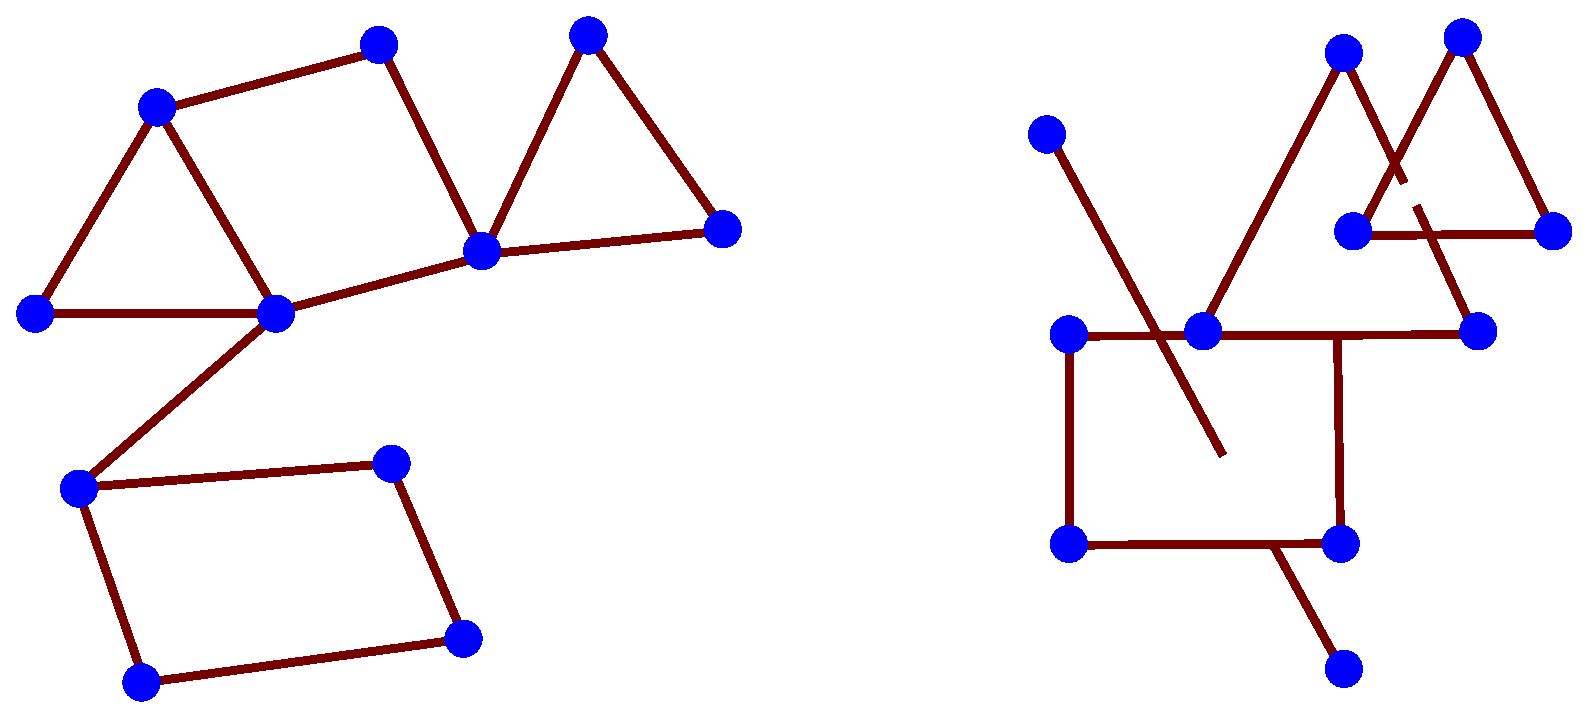
\includegraphics[angle=0,scale=0.3]{imagens/cap2/fig1.eps} \\
(a) \hspace{5.0cm} (b)\\
\caption{(a) Exemplo de complexo celular e (b) contra-exemplo de complexo celular.} 
\label{fig.celula}
\end{center}
\end{figure}


\begin{defi} $($Simplexo$)$
Uma c\'elula convexa afim 
$\sigma = [v_{0},\ldots,v_{k}]$ de $\R^{n}$ \'e chamada de simplexo, se 
$dim(\sigma) = k$, isto \'e, um simplexo $k$-dimensional \'e uma c\'elula 
convexa afim de dimens\~ao $k$ gerada por $k+1$ pontos. 
Um simplexo de dimensão 0 é denominado vértice e um simplexo de dimensão 1 é denominado aresta.
\end{defi}

\begin{defi} $($Triangulação$)$
Uma decomposi\c c\~ao celular $\mathcal{C}$ de 
$S \subset \R^{n}$ \'e chamada de triangula\c c\~ao de $S$, se
todas as c\'elulas de $\mathcal{C}$ s\~ao simplexos. 
\end{defi}

\begin{defi} $($Complexo Simplicial$)$
Um complexo simplicial é um complexo celular $\mathcal{C}$ onde todas as célula de $\mathcal{C}$ são simplexos.
\end{defi}

\begin{defi} $($Propriedades de Simplexos$)$
Dado um simplexo 
$\sigma = [v_{0}, \ldots, v_{k}]$ de $\R^{n}$, define-se : 
\begin{enumerate} 
\item A fronteira de $\sigma$, $\partial \sigma$, como a uni\~ao de todas as
      faces de dimens\~ao $k-1$ de $\sigma$; 
\item O baricentro de $\sigma$, $b(\sigma) = \frac{1}{k+1} \sum_{i=0}^{k}
      v_{i}$; 
\item O di\^ametro de $\sigma$, $\rho(\sigma) = max \{\parallel v_{i}-v_{j} 
\parallel; i, j = 0, \ldots, k\}$;
\item O raio de $\sigma$, $r(\sigma) = min \{\parallel v-b(\sigma) \parallel \; | \;
       v \in \partial(\sigma)\}$;
\item A robustez de $\sigma$, $\theta(\sigma) = r(\sigma)/\rho(\sigma)$.
\end{enumerate} 
\end{defi}

\begin{defi} $($Propriedades de Triangulação$)$
Se $T$ \'e uma triangula\c c\~ao de 
$S \subset \R^{n}$, define-se: 
\begin{enumerate} 
\item O di\^ametro de $T$, $\rho(T) = sup \{ \rho(\sigma) \; | \; \sigma \in T$ 
      com $dim(\sigma) > 0 \}$;
\item A robustez de $T$, $\theta(T) = inf \{ \theta(\sigma) \; | \; \sigma \in T$ 
      com $dim(\sigma) > 0 \}$.
\end{enumerate} 
\end{defi}

\begin{defi} $($Células Adjacentes$)$
Uma célula $\sigma_1$ é dita adjacente a outra célula $\sigma_2$ se $\sigma_1 \cap \sigma_2$ é uma face comum de $\sigma_1$ e $\sigma_2$.
\end{defi}

A Figura \ref{fig.adjacente} apresenta dois exemplos de adjacência entre células, um de células bidimensionais e outro de células tridimensionais.

\begin{figure}[h]
\begin{center} 
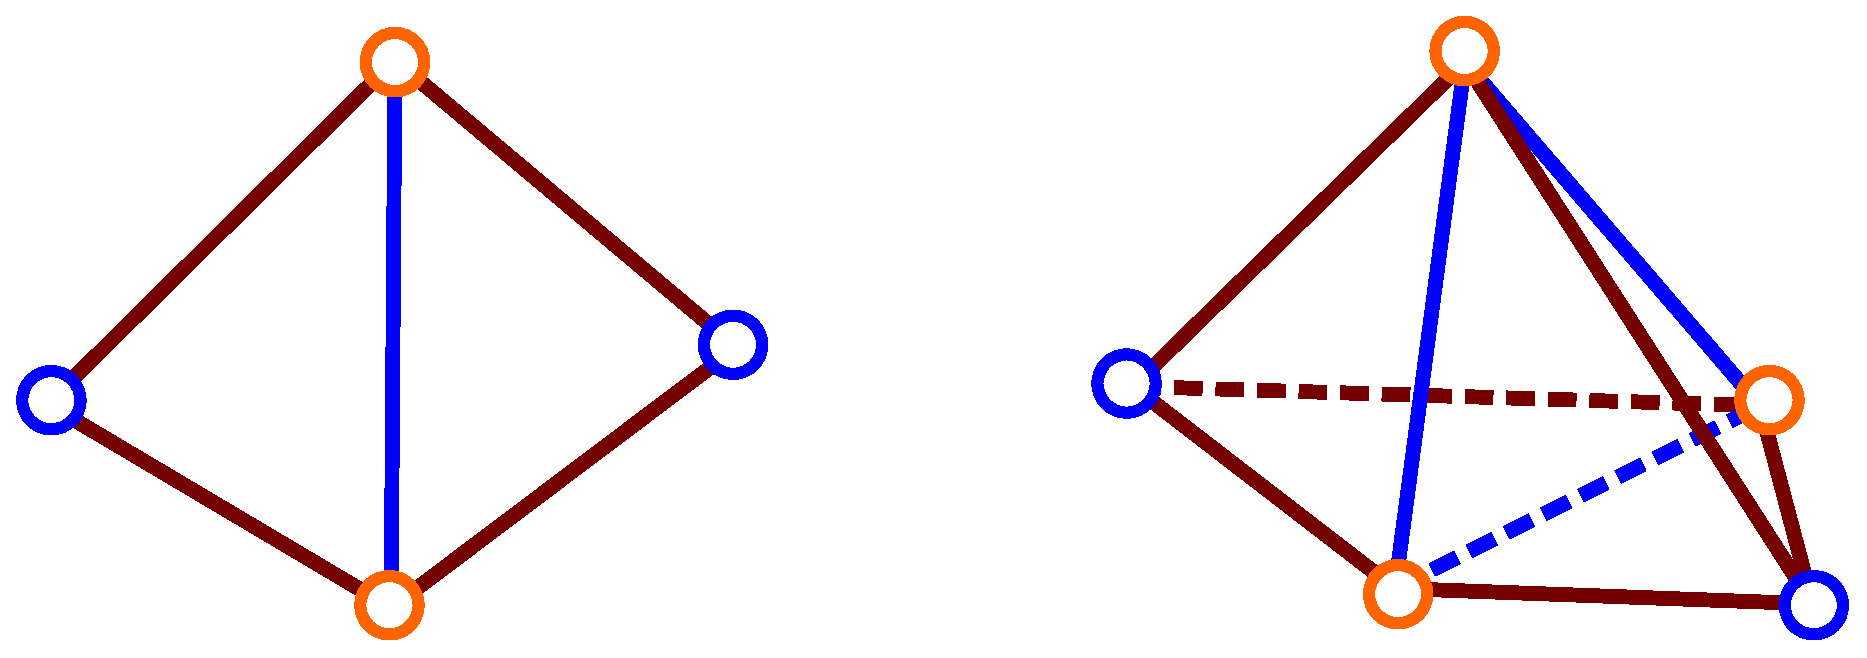
\includegraphics[angle=0,scale=0.3]{imagens/cap2/fig2.eps} \\
(a)Adjacência entre 2-células \hspace{1.cm} (b) Adjacência entre 3-células
\caption{Adjacências entre 2-células (por uma aresta) e 3-células (por uma face).} 
\label{fig.adjacente}
\end{center}
\end{figure}

\begin{defi} $($Vértices Vizinhos$)$
Um vértice é dito vizinho a outro se existe uma aresta que contém os dois.
\end{defi}

\begin{defi} $($Células Incidentes$)$
Dada uma célula $\sigma$ de dimensão $p$ e $\tau$ uma célula de dimensão $k$, onde $p > k$, estas células são ditas incidentes se $\tau$ é uma face de $\sigma$. 
\end{defi}

\begin{defi} $($Orientação de uma Célula$)$
Seja $\mathcal{C}$ um complexo celular de dimensão $p$, onde $p$ é a maior dimensão de todas as células. A orientação de duas células adjacentes $\sigma$ e $\tau$ de dimensão $p$ de $\mathcal{C}$ é coerente se face de dimensão $p-1$ que compartilham tem orientação oposta em cada uma das células. O complexo celular $\mathcal{C}$ é orientável se uma orientação coerente pode ser escolhida para todas as suas células.
\end{defi}


\begin{figure}[h]
\begin{center} 
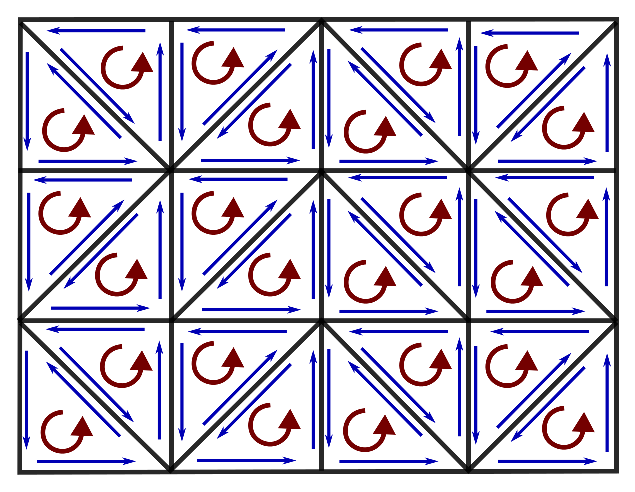
\includegraphics[angle=0,scale=0.7]{imagens/cap2/fig3.eps}
\caption{Complexo celular bidimensional orientado em sentido anti-horário.} 
\label{fig.orientacao}
\end{center}
\end{figure}


\begin{defi} $($Estrela de uma Célula$)$
A estrela de uma célula $\sigma$ de um complexo celular $\mathcal{C}$, denominada por $S(\sigma)$ é o conjunto de todas as células de $\mathcal{C}$ que contém $\sigma$, isto é, $S(\sigma) = \{ \tau \in \mathcal{C} \; | \; \sigma \subseteq \tau \}$.
\end{defi}

\begin{defi} $($Elo de uma Célula$)$
O elo de uma célula $\sigma \subset \mathcal{C}$ é o conjunto $L(\sigma) = \{ \tau \in \overline{S(\sigma)} \; | \; \tau \cap \sigma = \emptyset \}$, onde $\overline{S(\sigma)}$ é o fecho da estrela de $\sigma$.
\end{defi}

Um exemplo de estrela e de elo de um vértice central é mostrado na Figura \ref{fig.elo}(b). 

\begin{figure}[h]
\begin{center} 
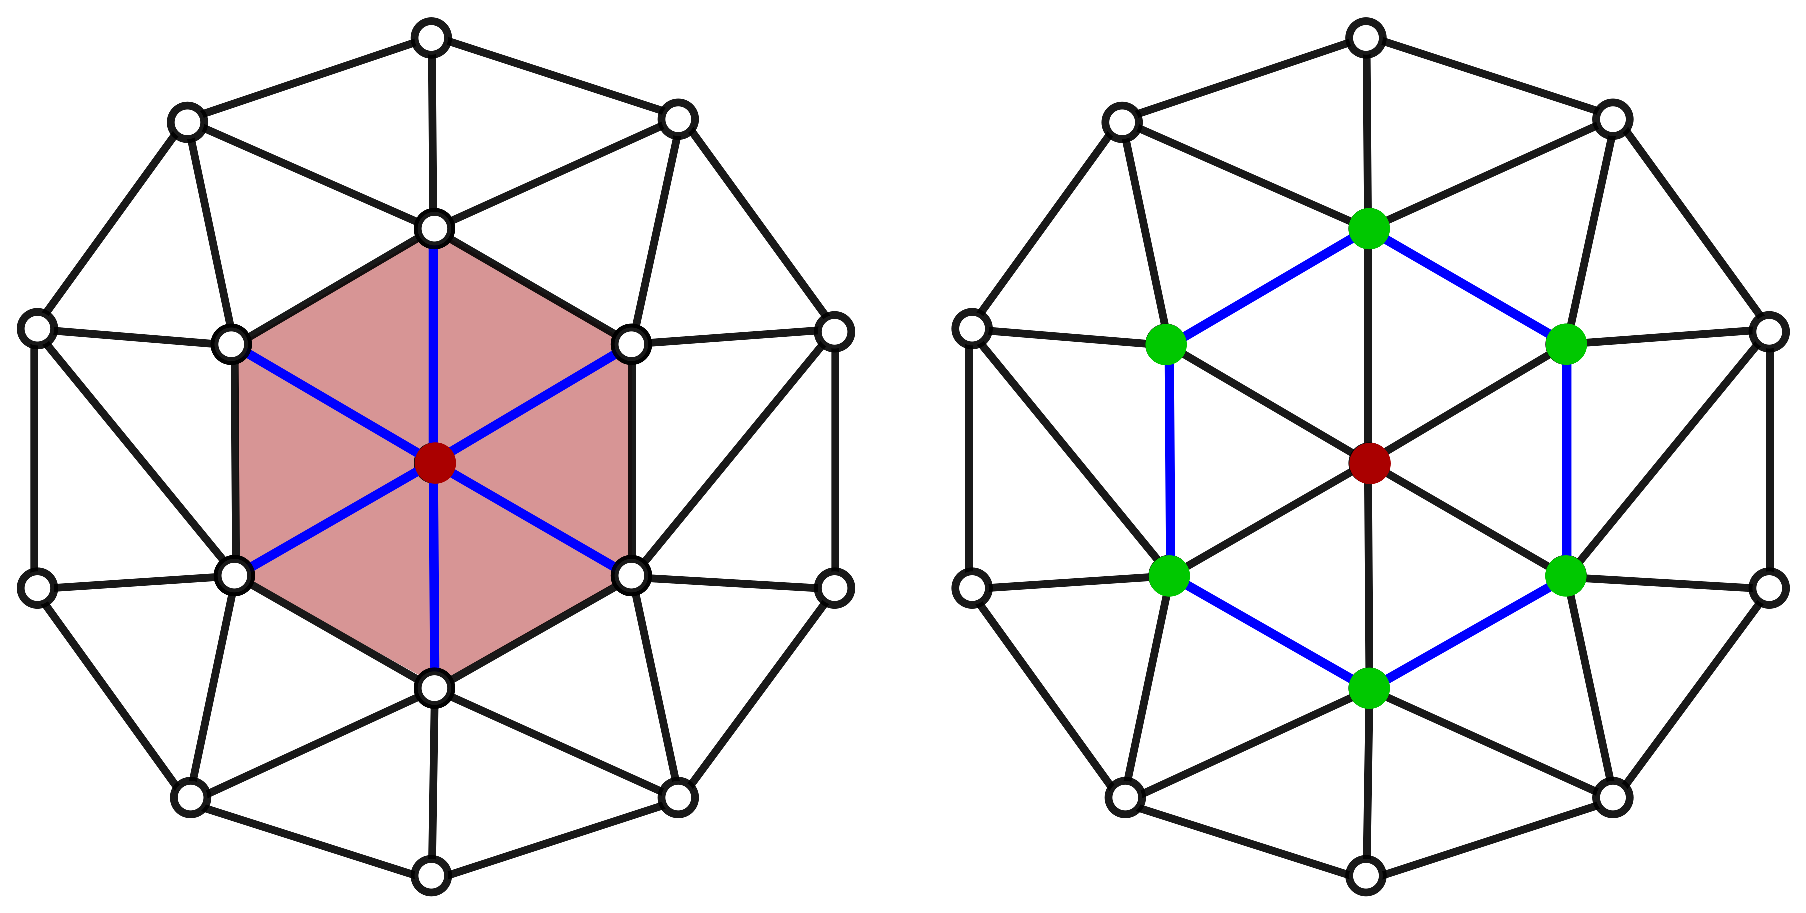
\includegraphics[angle=0,scale=0.3]{imagens/cap2/fig4.eps}\\
(a) Estrela do vértice central \hspace{1.0cm} (b) Elo do vértice central\\
\caption{Representações de uma estrela e um elo de um vértice.} 
\label{fig.elo}
\end{center}
\end{figure}


\begin{defi} $($Variedade Linear por Partes$)$
Um complexo celular $\mathcal{C}$ de dimensão $n$ é dito uma variedade linear por partes de dimensão $n$ se para todo $\sigma \in \mathcal{C}$, ou $L(\sigma)$ é homeomorfo a uma esfera de dimensão $n-1$, ou é homeomorfo a um disco de dimensão $n-1$. 
Caso $L(\sigma)$ seja homeomorfo a um disco de dimensão $n-1$, $\sigma$ pertence ao bordo de $\mathcal{C}$. 
\end{defi}


A figura \ref{fig.varLinPartes}-(a) dá um exemple de um vértice de interior, enquanto a figura \ref{fig.varLinPartes}-(b) exemplifica um vértice de bordo de uma variedade linear por partes de dimensão 2. 
Já a figura \ref{fig.varLinPartes}-(c) exibe uma não-variedade. 

\begin{figure}[h]
\begin{center} 
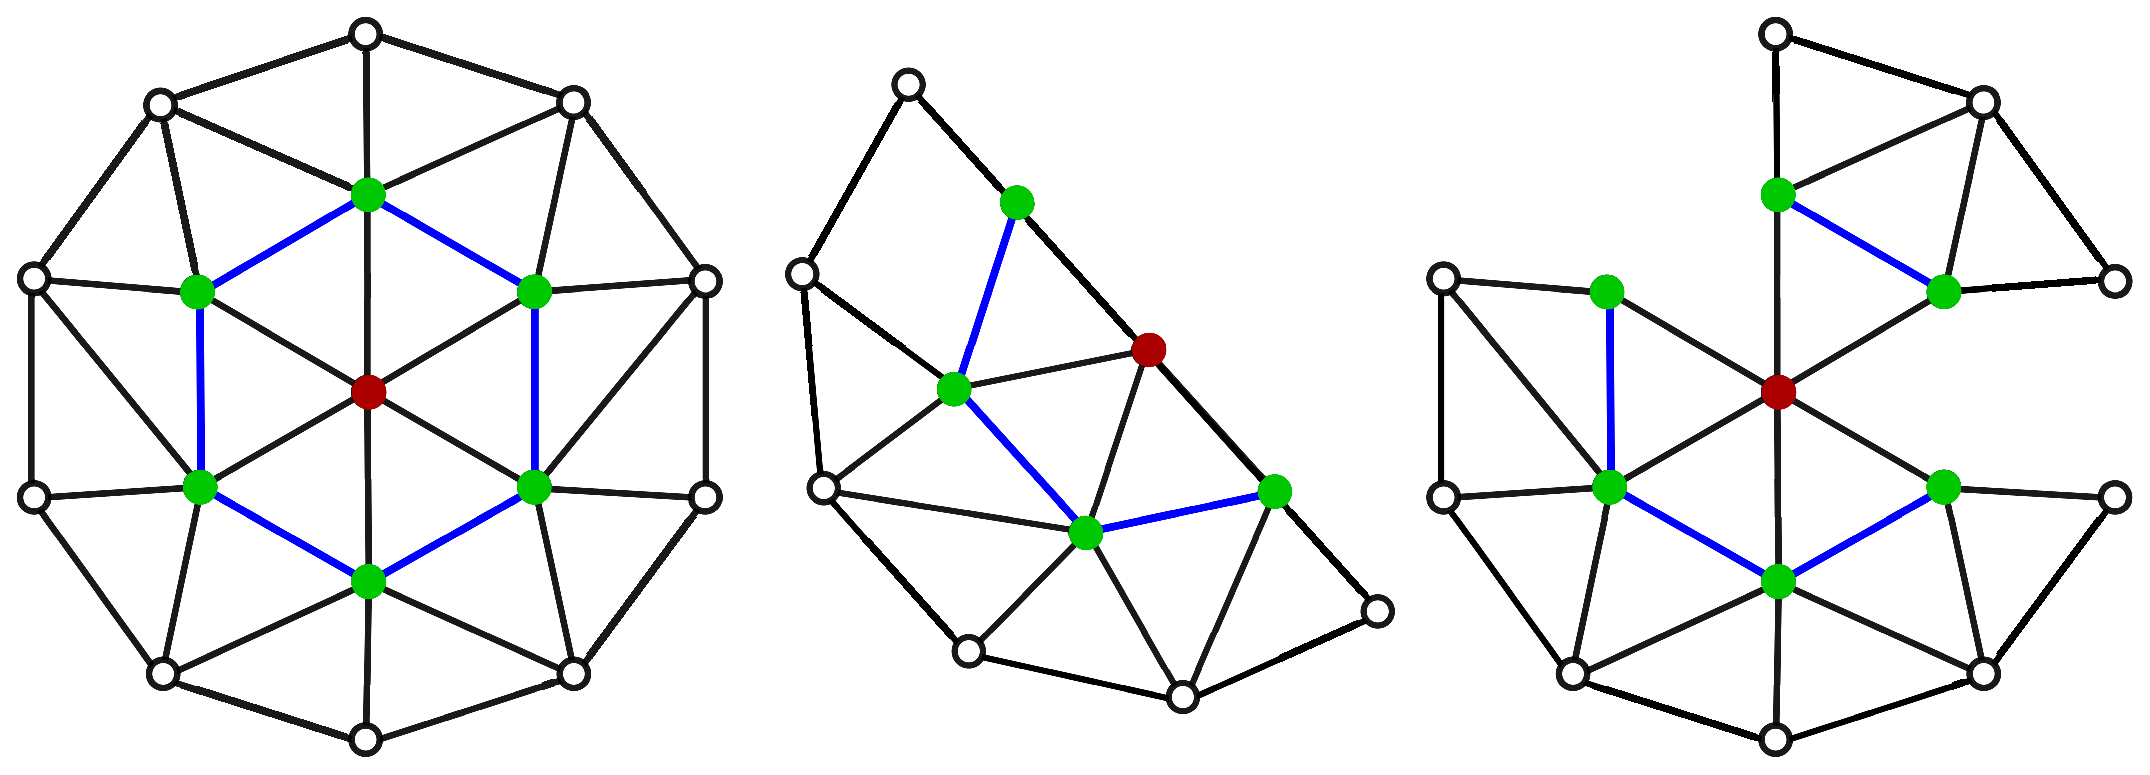
\includegraphics[angle=0,scale=0.3]{imagens/cap2/fig5.eps}\\
(a) Ponto de interior \hspace{0.8cm} (b) Ponto de Bordo \hspace{0.8cm} (c) Não-variedade
\caption{Exemplos de variedades (a) e (b) e de não-variedade (c).} 
\label{fig.varLinPartes}
\end{center}
\end{figure}

\begin{defi} $($Variedade Triangulada$)$
Uma variedade triangulada $\mathcal{C}$ é uma variedade linear por partes onde todas suas células são simplexos.
\end{defi}




\markboth{Variedades}{Formas de Representação de Variedades}
\section{Formas de Representação de Variedades}\label{var_formas}

As formas de representação mais comuns de variedades são como gráfico de uma função, a imagem de uma função e como a imagem inversa de uma função.
Estas formas de reapresentação serão definidas e exemplificadas nas próximas subseções.


\markboth{Variedades}{Variedades como Gráfico de Funções}
\subsection{Variedades como Gráfico de Funções}\label{var_grafico}


Seja $F: U \subset \R^n \rightarrow \R$ de classe $C^r$. O conjunto
$\mathcal{M} = \{ \; (x,F(x)) \; | \; x \in U \; \}$ é uma variedade de dimensão $n$ em $\R^{n+1}$ de classe $C^r$.
Neste caso $\mathcal{M}$ é o gráfico da função $F$.

Os casos mais simples s\~ao:
\begin{itemize}
 \item Para $n=1$ o gráfico de $F$ \'e uma curva em $\R^2$;
 \item Para $n=2$ o gráfico de $F$ \'e uma superf\'icie em $\R^3$.
\end{itemize}

\noindent {\bf Exemplo 1:} Como exemplo de curva em $\R^2$, apresentamos o código \ref{senocoseno} em Matlab/Octave com o gráfico das funções cosseno e seno. A figura \ref{fig.CosSin} apresenta o resultado da execução deste código. 

\begin{Codigo}[htpb]
\noindent\rule{13cm}{1.pt}
\begin{verbatim}
x  = linspace(0,2*pi,30);              % gerando os pontos do domínio
y1 = cos(x);                           % gerando a função cosseno 
y2 = sin(x);                           % gerando a função seno 
hold on
plot(x,y1,'r-s');                      % plotando o gráfico do cosseno
plot(x,y2,'g-*');                      % plotando o gráfico do seno
grid                                   % gerando um grid
xlabel('eixo x');                      % legenda no eixo horizontal
ylabel('eixo y');                      % legenda no eixo vertical
title('Grafico do seno e do cosseno'); % título do gráfico 
legend('sen(x)','cos(x)');             % legenda
hold off
\end{verbatim}
\vspace{-0.5cm}
\caption{Código utilizado para gerar a figura \ref{fig.CosSin} } 
\noindent\rule{13cm}{1.pt}
\label{senocoseno}
\end{Codigo}

\begin{figure}[htpb]
\begin{center} 
\psfrag{Grafico do seno e do cosseno}[c][c][2.3]{\textbf{Gráfico do seno e do cosseno}}
\psfrag{sen(x)}[c][c][1.1]{\hspace{-0.1cm} $cos(x)$}
\psfrag{cos(x)}[c][c][1.1]{\hspace{-0.1cm} $sin(x)$}
\psfrag{eixo x}[c][c][2.3]{eixo $x$}
\psfrag{eixo y}[b][b][2.3]{eixo $y$}
\includegraphics*[angle=0,scale=0.5]{imagens/cap2/CosSin.eps} 
\vspace{-0.5cm}
\caption{Curvas em $\R^2$ geradas como gráfico das funções cosseno e seno.} 
\label{fig.CosSin}
\end{center}
\end{figure}

\noindent {\bf Exemplo 2:} Como exemplo de superfície em $\R^3$, apresentamos o gráfico da função $z=F(x,y)=\frac{sen(\sqrt{x^2+y^2}+0.1)}{\sqrt{x^2+y^2}+0.1}$. A figura \ref{fig.3d_1} apresenta o resultado da execução do código \ref{fig3d} feito em Matlab/Octave.

\begin{Codigo}[htpb]
\noindent\rule{13cm}{1.pt}
\begin{verbatim}
px = py = linspace (-10, 10, 50)';     % gerando os pontos do domínio
[x, y] = meshgrid (px, py);            % criando a malha 
r = sqrt(x.^2 + y.^2) + 0.1;           % r é variável auxiliar
z = sin(r) ./ r;                       % função z=F(x,y) 
surf (x, y, z);                        % plotando a superfície
xlabel('eixo x');                      % legenda no eixo x
ylabel('eixo y');                      % legenda no eixo y
zlabel('F(x,y)');                      % legenda no eixo z
title('Exemplo de Superficie');        % título do gráfico 
legend('Superficie z=F(x,y)');         % legenda
\end{verbatim}
\vspace{-0.5cm}
\caption{Código utilizado para gerar a figura \ref{fig.3d_1} } 
\noindent\rule{13cm}{1.pt}
\label{fig3d}
\end{Codigo}

\begin{figure}[htpb]
\begin{center} 
\psfrag{Exemplo de Superficie}[c][c][2.3]{\textbf{Exemplo de Superfície}}
\psfrag{Superficie z=F(x,y)}[c][c][1.0]{\hspace{0.3cm} Superfície $z=F(x,y)$}
\psfrag{eixo x}[c][c][2.3]{eixo $x$}
\psfrag{eixo y}[c][c][2.3]{eixo $y$}
\psfrag{F(x,y)}[b][b][2.]{$F(x,y)$}
\includegraphics*[angle=0,scale=0.55]{imagens/cap2/superficie.eps}
\caption{Superfície dada pela função $F(x,y)=\frac{sen(\sqrt{x^2+y^2}+0.1)}{\sqrt{x^2+y^2}+0.1}$} 
\label{fig.3d_1}
\end{center}
\end{figure}

Substituindo o comando {\it surf} pelo comando {\it mesh} obtemos o gráfico $z=F(x,y)$ apenas nos pontos do {\it grid} do domínio. A figura \ref{fig.3d_2} apresenta o resultado usando mesh (ver código  \ref{mesh}).


\begin{Codigo}[htpb]
\noindent\rule{13cm}{1.pt}
\begin{verbatim}
px = py = linspace (-10, 10, 50)';     % gerando os pontos do domínio
[x, y] = meshgrid (px, py);            % criando a malha 
r = sqrt(x.^2 + y.^2) + 0.1;           % r é variável auxiliar
z = sin(r) ./ r;                       % função z=F(x,y) 
mesh (x, y, z);                        % plotando a superfície
xlabel('eixo x');                      % legenda no eixo x
ylabel('eixo y');                      % legenda no eixo y
zlabel('F(x,y)');                      % legenda no eixo z
title('Exemplo de Superficie');        % título do gráfico 
legend('Superficie z=F(x,y)');         % legenda
\end{verbatim}
\vspace{-0.5cm}
\caption{Código utilizado para gerar a figura \ref{fig.3d_2} } 
\noindent\rule{13cm}{1.pt}
\label{mesh}
\end{Codigo}

\begin{figure}[htpb]
\begin{center} 
\psfrag{Exemplo de Superficie}[c][c][2.3]{\textbf{Exemplo de Superfície}}
\psfrag{Superficie z=F(x,y)}[c][c][1.0]{\hspace{0.3cm} Superfície $z=F(x,y)$}
\psfrag{eixo x}[c][c][2.3]{eixo $x$}
\psfrag{eixo y}[c][c][2.3]{eixo $y$}
\psfrag{F(x,y)}[b][b][2.]{$F(x,y)$}
\includegraphics*[angle=0,scale=0.55]{imagens/cap2/malha.eps} 
\caption{Superfície gerada pela função $F(x,y)=\frac{sen(\sqrt{x^2+y^2}+0.1)}{\sqrt{x^2+y^2}+0.1}$ nos pontos do {\it grid}} 
\label{fig.3d_2}
\end{center}
\end{figure}

\newpage 

\markboth{Variedades}{Variedades Parametrizadas}
\subsection{Variedades Parametrizadas}\label{var_param}

Seja $F: U \subset \R^k \rightarrow \R^n$, $ n \geq k$, de classe $C^r$. O conjunto
$\mathcal{M} = \{ \; F(x) \; | \; x \in U \; \}$ é uma variedade de dimensão $k$ em $\R^{n}$ de classe $C^r$.
Neste caso $\mathcal{M}$ é a imagem da função $F$, e $F$ é denominada parametrização de $\mathcal{M}$.

As parametrizações mais comuns são tratadas nos curso de c\'alculo e geometria diferencial:
\begin{itemize}
 \item Para $n=2$ e $k=1$, $F(x)$ \'e uma curva em $\R^2$;
 \item Para $n=3$ e $k=1$, $F(x)$ \'e uma curva em $\R^3$;
 \item Para $n=3$ e $k=2$, $F(x)$ \'e uma superf\'icie em $\R^3$.
\end{itemize}

\noindent {\bf Exemplo 1:} Uma exemplo de curva parametrizada em $\R^2$ é apresentada  em \ref{fig.pplanacurva} e foi gerada pelo código \ref{pplanacurva} em Matlab/Octave.

\begin{Codigo}[htpb]
\noindent\rule{13cm}{1.pt}
\begin{verbatim}
t = linspace(-2,2,80);                   % intervalo do parâmetro t
f = @(t) t.^2+1.0;                       % gerando a função f
g = @(t) t.*cos(t);                      % gerando a função g 
plot(f(t), g(t));                        % plotando 
grid                                     % gerando um grid
xlabel('f(t)');                          % legenda no eixo horizontal
ylabel('g(t)');                          % legenda no eixo vertical
title('Exemplo de curva Parametrizada'); % título do gráfico 
legend('Curva F(t)=(f(t),g(t))');        % legenda
\end{verbatim}
\vspace{-0.5cm}
\caption{Código utilizado para gerar a figura \ref{fig.pplanacurva} } 
\noindent\rule{13cm}{1.pt}
\label{pplanacurva}
\end{Codigo}


\begin{figure}[htpb]
\begin{center} 
\psfrag{Exemplo de curva Parametrizada}[c][c][2.3]{\textbf{Exemplo de curva parametrizada}}
\psfrag{Curva F(t)= < f(t), g(t) >}[c][c][1.1]{\hspace{0.5cm} Curva $F(t)=(f(t),g(t))$}
\psfrag{f(t)}[c][c][2.3]{$f(t)$}
\psfrag{g(t)}[b][b][2.]{$g(t)$}
\includegraphics*[angle=0,scale=0.5]{imagens/cap2/pplanacurva.eps}
\caption{Curva $F(t) = (t^2+1, t\ cos(t))$, $t=[-2:2]$} 
\label{fig.pplanacurva}
\end{center}
\end{figure}

\noindent {\bf Exemplo 2:} Como exemplo de curva parametrizada em $\R^3$, apresentamos o código em Matlab/Octave \ref{pespcurva}. A figura \ref{fig.pespcurva} apresenta o resultado da execução deste código.

\begin{Codigo}[htpb]
\noindent\rule{13cm}{1.pt}
\begin{verbatim}
t = linspace(0,20,100);                     % intervalo do parâmetro t
plot3(sin(t),cos(t),t);                     % plotando 
grid                                        % gerando um grid
xlabel('eixo x')                            % legenda no eixo x
ylabel('eixo y')                            % legenda no eixo y
zlabel('eixo z')                            % legenda no eixo z
axis square
title('Exemplo de curva Parametrizada');         % título do gráfico 
legend('Curva F(t)=(sin(t),cos(t),t),t=[0,20]'); % legenda
\end{verbatim}
\vspace{-0.5cm}
\caption{Código utilizado para gerar a figura \ref{fig.pespcurva} } 
\noindent\rule{13cm}{1.pt}
\label{pespcurva}
\end{Codigo}

\begin{figure}[htpb]
\begin{center}
\psfrag{Exemplo de curva Parametrizada}[c][c][2.3]{\textbf{Exemplo de curva parametrizada}}
\psfrag{Curva F(t)=< sin(t), cos(t), t>, t=[0,20]}[c][c][1.1]{\hspace{0.85cm} Curva $F(t)=(sin(t),cos(t),t), t=[0,20]$}
\psfrag{eixo x}[c][c][2.3]{$eixo \ x$}
\psfrag{eixo y}[c][c][2.3]{$eixo \ y$}
\psfrag{eixo z}[b][b][2.0]{$eixo \ z$}
\includegraphics*[angle=0,scale=0.5]{imagens/cap2/pespcurva.eps} 
\caption{Curva em $\R^3$ da função $F(t)= (sin(t), cos(t), t)$ , $t=[0,20]$ } 
\label{fig.pespcurva}
\end{center}
\end{figure}

\noindent {\bf Exemplo 3:}  Como exemplo de superfície parametrizada em $\R^3$, apresentamos o código em Matlab/Octave \ref{pespsurf}. A figura \ref{fig.pespsurf} apresenta o resultado da execução deste código.

\begin{Codigo}[htpb]
\noindent\rule{13cm}{1.pt}
\begin{verbatim}
t = linspace(0,10,40);                      % intervalo do parâmetro t 
u = linspace(-2,2,40);                      % intervalo do parâmetro u
[t,u] = meshgrid(t,u);                      % gerando a malha
x = 2.*t;                                   % f(t,u)
y = 3*u.*cos(t);                            % g(t,u)
z = u.*sin(t);                              % h(t,u)
surf(x,y,z);                                % plotando
xlabel('eixo x')                            % legenda no eixo x
ylabel('eixo y')                            % legenda no eixo y
zlabel('eixo z')                            % legenda no eixo z
axis square
title('Exemplo de Superfície Parametrizada');  % título do gráfico 
legend('Superficie F(t,u)');                   % legenda
\end{verbatim}
\vspace{-0.5cm}
\caption{Código utilizado para gerar a figura \ref{fig.pespsurf} } 
\noindent\rule{13cm}{1.pt}
\label{pespsurf}
\end{Codigo}

\begin{figure}[htpb]
\begin{center} 
\psfrag{Exemplo de Superficie Parametrizada}[c][c][2.3]{\textbf{Exemplo de superfície parametrizada}}
\psfrag{Superficie F(t,u)}[c][c][1.1]{\hspace{0.25cm} Superfície  $F(t,u)$}
\psfrag{eixo x}[c][c][2.3]{$eixo \ x$}
\psfrag{eixo y}[c][c][2.3]{$eixo \ y$}
\psfrag{eixo z}[b][b][2.0]{$eixo \ z$}
\includegraphics*[angle=0,scale=0.5]{imagens/cap2/pespsurf.eps} 
\caption{Superfície $F(t,u) = (f(t,u), g(t,u), h(t,u))$, $t=[0,10]$, $u=[-2,2]$, $f(t,u)=2\ t$, $g(t,u)=3\ u\ cos(t)$, $h(t,u)=u\ sen(t)$.} 
\label{fig.pespsurf}
\end{center}
\end{figure}

Substituindo o comando {\it surf} pelo comando {\it mesh} (ver código \ref{pespmesh}) obtemos o gráfico anterior apenas nos pontos do {\it grid} do domínio (ver  figura \ref{fig.pespmesh}). 

\begin{Codigo}[htpb]
\noindent\rule{13cm}{1.pt}
\begin{verbatim}
t = linspace(0,10,40);                     % intervalo do parâmetro t 
u = linspace(-2,2,40);                     % intervalo do parâmetro u
[t,u] = meshgrid(t,u);                     % gerando a malha
x = 2.*t;                                  % f(t,u)
y = 3*u.*cos(t);                           % g(t,u)
z = u.*sin(t);                             % h(t,u)
mesh(x,y,z);                               % plotando
xlabel('eixo x')                           % legenda no eixo x
ylabel('eixo y')                           % legenda no eixo y
zlabel('eixo z')                           % legenda no eixo z
axis square
title('Exemplo de Superfície Parametrizada');  % título do gráfico 
legend('Superficie F(t,u)');                   % legenda
\end{verbatim}
\vspace{-0.5cm}
\caption{Código utilizado para gerar a figura \ref{fig.pespmesh}} 
\noindent\rule{13cm}{1.pt}
\label{pespmesh}
\end{Codigo}

\begin{figure}[htpb]
\begin{center} 
\psfrag{Exemplo de Superficie Parametrizada}[c][c][2.3]{\textbf{Exemplo de superfície parametrizada}}
\psfrag{Superficie F(t,u)}[c][c][1.1]{\hspace{0.25cm} Superfície  $F(t,u)$}
\psfrag{eixo x}[c][c][2.3]{$eixo \ x$}
\psfrag{eixo y}[c][c][2.3]{$eixo \ y$}
\psfrag{eixo z}[b][b][2.0]{$eixo \ z$}
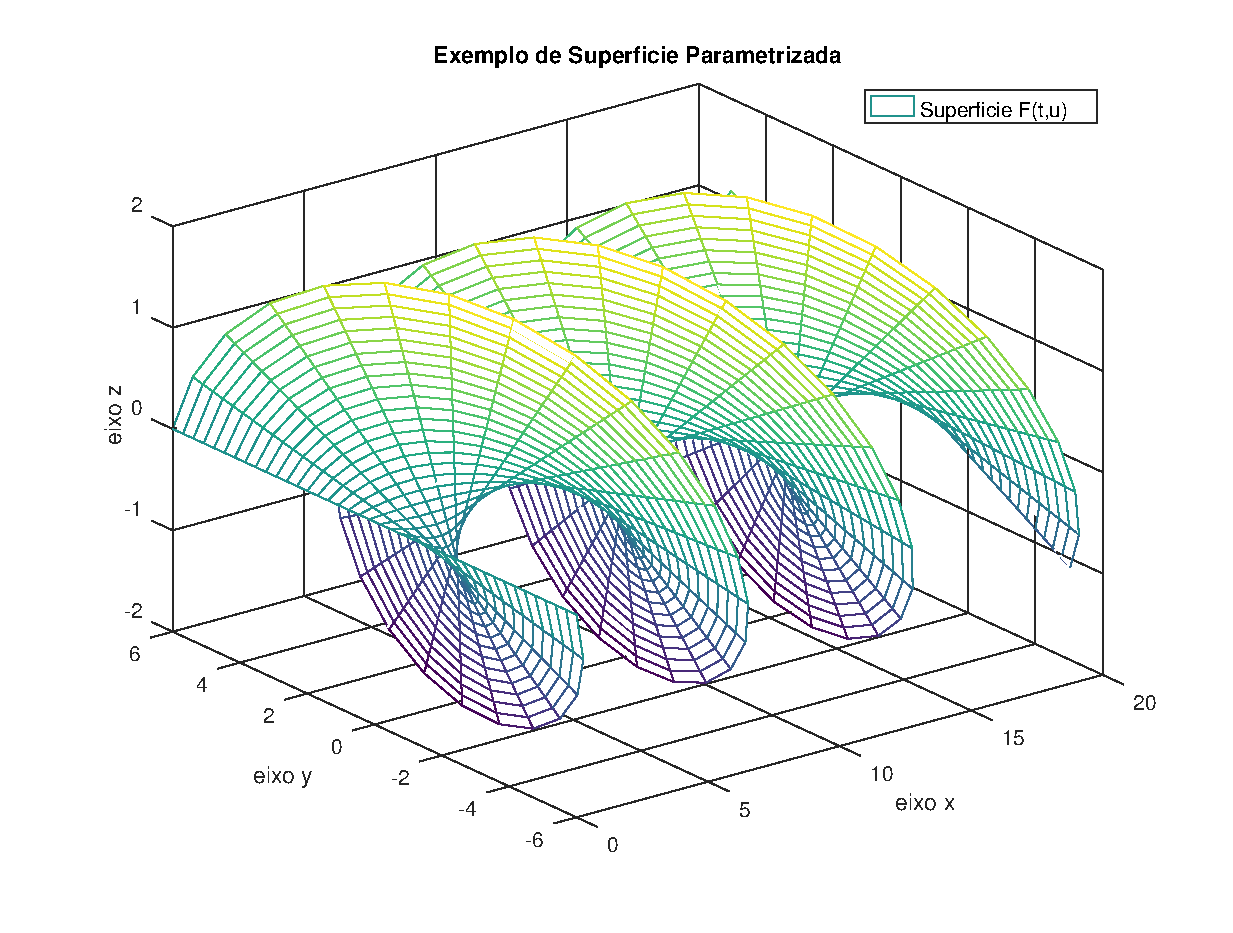
\includegraphics[angle=0,scale=0.5]{imagens/cap2/pespmesh.eps} 
\caption{Superfície $F(t,u) = (f(t,u), g(t,u), h(t,u))$, $t=[0,10]$, $u=[-2,2]$, $f(t,u)=2\ t$, $g(t,u)=3\ u\ cos(t)$, $h(t,u)=u\ sen(t)$ nos pontos de {\it grid}.} 
\label{fig.pespmesh}
\end{center}
\end{figure}

\newpage
\newpage

\markboth{Variedades}{Variedades Definidas Implicitamente}
\subsection{Variedades Definidas Implicitamente}\label{var_impl}

Dada uma fun\c{c}\~ao de classe $C^r$, $F : \R^n \rightarrow \R^k$, $n \geq k$,  o conjunto dos pontos onde $F$ se anula $\mathcal{M} = F^{-1}(0) = \{ x \in \R^n  \; | \: F(x) = 0 \}$, \'e uma variedade definida implicitamente se para todo ponto em $\mathcal{M}$ a derivada de $F$ neste ponto tem posto m\'aximo. Neste caso a variedade $\mathcal{M}$ tem dimens\~ao $n-k$ (veja o Teorema \ref{teo_VI} da Se\c{c}\~ao \ref{var_dif}). 

Os casos mais comuns geralmente vistos nos cursos de c\'alculo s\~ao:
\begin{itemize}
 \item Para $n=2$ e $k=1$, $F^{-1}(0)$ \'e uma curva em $\R^2$;
 \item Para $n=3$ e $k=2$, $F^{-1}(0)$ \'e uma curva em $\R^3$;
 \item Para $n=3$ e $k=1$, $F^{-1}(0)$ \'e uma superf\'icie em $\R^3$.
\end{itemize}


\noindent {\bf Exemplo 1:} Seja $f:\R^2 \rightarrow \R$ dada por  $F(x,y)=3.5^{-\sqrt{x^2+y^2}} cos(y) sin(x/2)$. A variedade $\mathcal{M}$ é representada na figura \ref{fig.projecao}-(a) e foi gerada usando o código \ref{supcurvanivel} feito em Matlab/Octave. A figura \ref{fig.projecao}-(b) foi gerada usando o código \ref{supcurvanivelb} e mostra o gráfico de $F(x,y)$ e sua projeção.

\begin{Codigo}[htpb]
\noindent\rule{13cm}{1.pt}
 \begin{verbatim}
px = py = linspace (-3, 3, 50)';                    % domínio
[x, y] = meshgrid (px, py);                         % gerando a malha
z = 3.5.^(-1.*sqrt(x.^2+y.^2)).*cos(y).*sin(0.5*x); % superficie z=f(x,y)
contour(x,y,z,10)                                   % 10 curvas de nível
xlabel('eixo x')                                    % legenda no eixo x
ylabel('eixo y')                                    % legenda no eixo y
legend('Plano xy');                                 % legenda
\end{verbatim} 
\caption{Código utilizado para gerar a figura \ref{fig.projecao}-(a) } 
\noindent\rule{13cm}{1.pt}
\label{supcurvanivel}
\end{Codigo}

\begin{Codigo}[htpb]
\noindent\rule{13cm}{1.pt}
\begin{verbatim}
px = py = linspace (-3, 3, 50)';                  % domínio
[x, y] = meshgrid (px, py);                       % gerando a malha
z=3.5.^(-1.*sqrt(x.^2+y.^2)).*cos(y).*sin(0.5*x); % superficie z=f(x,y)
surfc(x,y,z)                                      % plotando o grafico 
                                                  % de F(x,y) e algumas 
                                                  % curvas de nível
xlabel('eixo x')                                  % legenda no eixo x
ylabel('eixo y')                                  % legenda no eixo y
zlabel ('F(x,y)')                                 % legenda no eixo z
title('Exemplo de Superficie');                   % título
legend('Superficie z=F(x,y)');                    % legenda                          
\end{verbatim}
\caption{Código utilizado para gerar a figura \ref{fig.projecao}-(b) } 
\noindent\rule{13cm}{1.pt}
\label{supcurvanivelb}
\end{Codigo}



\begin{figure}[htpb]
\begin{tabular}{cc}
\hspace{-2.0cm}
\psfrag{Plano xy}[c][c][1.1]{\hspace{0.15cm} Plano $xy$}
\psfrag{eixo x}[c][c][2.3]{$eixo \ x$}
\psfrag{eixo y}[b][b][2.0]{$eixo \ y$}
\includegraphics*[angle=0,scale=0.5]{imagens/cap2/projecao.eps} & 
 \psfrag{Exemplo de Superficie}[c][c][2.3]{\textbf{Exemplo de superfície}}
\psfrag{Superficie z=F(x,y)}[c][c][1.0]{\hspace{0.25cm} Superfície  $z=F(x,y)$}
\psfrag{eixo x}[c][c][2.3]{$eixo \ x$}
\psfrag{eixo y}[c][c][2.3]{$eixo \ y$}
\psfrag{F(x,y)}[b][b][2.0]{$F(x,y)$}
\hspace{-1.4cm}
\includegraphics*[angle=0,scale=0.4]{imagens/cap2/projxy.eps} \\
(a) & (b) 
\end{tabular}
\caption{Superficie $F(x,y)=3.5^{-\sqrt{x^2+y^2}} cos(y) sin(x/2)$.}
\label{fig.projecao}
\end{figure}



\noindent {\bf Exemplo 2:} Seja $f:\R^3 \rightarrow \R$ dada por $f(x, y, z) = x^2 + y^2 + z^2$ . A esfera {$S^2$} de raio $r=2$ fica definida implicitamente pela equação $f(x,y,z) = 4$. A figura \ref{fig.esfera} mostra a Isosuperfície gerada pelo código abaixo, feito em Matlab/Octave

\begin{Codigo}[htpb]
\noindent\rule{13cm}{1.pt}
\begin{verbatim}
[x,y,z] = meshgrid(-2:0.2:2,-2:0.2:2,-2:0.2:2); % gerando a malha
F = x.^2 + y.^2 + z.^2 -4.0 ;                   % esfera 
isosurface(x,y,z,F,0);                          % isosuperfície
axis equal;
xlabel('eixo x')                                % legenda no eixo x
ylabel('eixo y')                                % legenda no eixo y
zlabel('eixo z')                                % legenda no eixo z
legend('Esfera');                               % legenda
\end{verbatim}
\caption{Código utilizado para gerar a figura \ref{fig.esfera}} 
\noindent\rule{13cm}{1.pt}
\label{esfera}
\end{Codigo}


\begin{figure}[htpb]
\begin{center} 
\psfrag{Esfera raio 2}[c][c][1.0]{\hspace{0.25cm} Esfera raio $2$}
\psfrag{eixo x}[c][c][2.3]{$eixo \ x$}
\psfrag{eixo y}[c][c][2.3]{$eixo \ y$}
\psfrag{eixo z}[c][c][2.3]{$eixo \ z$}
\includegraphics*[angle=0,scale=0.5]{imagens/cap2/esfera_isosurf.eps} 
\caption{Isosuperfície $F(x,y,z)=x^2+y^2+z^2-4.0$} 
\label{fig.esfera}
\end{center}
\end{figure}


\noindent {\bf Exemplo 3:} Seja $F:\R^3 \rightarrow \R^2$ dada por $F(x,y,z) = (f_1(x,y,z),f_2(x,y,z))$, onde $f_1(x,y,z)= x^2 + y^2 + z^2 - 1$ e $f_2(x,y,z)= 2x^2 + 2y^2 - 1$.
O conjunto $f_1^{-1}(0)$ é a esfera {$S^2$} de raio $r=1$ e o conjunto $f_2^{-1}(0)$ é um cilindro. 
A figura \ref{fig.isosurfr3r2}-(a) mostra as isosuperfícies gerada pelo código, feito em Matlab/Octave. Neste caso, $F^{-1}({\bf 0})=f_1^{-1}(0)\bigcap f_2^{-1}(0)$ são os círculos nos planos $z=\sqrt{2}$ e $z=-\sqrt{2}$ mostrados na figura \ref{fig.isosurfr3r2}-(b). 

\begin{Codigo}[htpb]
\noindent\rule{13cm}{1.pt}
\begin{verbatim}
[x,y,z] = meshgrid(-2:0.2:2,-2:0.2:2,-2:0.2:2); % gerando a malha
f1 = x.^2 + y.^2 + z.^2 -1.0 ;                  % esfera
f2 =2.0.*x.^2 + 2.0.*y.^2 -1.0 ;                % cilindro                        
isosurface(x,y,z,f1,0.1);                       % isosuperfície
isosurface(x,y,z,f2,0);                         % isosuperfície
camlight;
lighting gouraud;
axis equal;
xlabel('eixo x')                                % legenda no eixo x
ylabel('eixo y')                                % legenda no eixo y
zlabel('eixo z')                                % legenda no eixo z
\end{verbatim}
\caption{Código utilizado para gerar a figura \ref{fig.isosurfr3r2}} 
\noindent\rule{13cm}{1.pt}
\label{isosurfr3r2}
\end{Codigo}


\begin{figure}[htpb]
\begin{tabular}{cc}
\hspace{-3.3cm}
 \psfrag{eixo x}[c][c][2.3]{$eixo \ x$}
\psfrag{eixo y}[c][c][2.3]{$eixo \ y$}
\psfrag{eixo z}[b][b][2.3]{$eixo \ z$}
\includegraphics*[angle=0,scale=0.5]{imagens/cap2/isosurfr3r2.eps} & 
\hspace{-3.2cm}\includegraphics*[angle=0,scale=0.36]{imagens/cap2/isosurfr3r2_2.eps} \\
\hspace{-3.3cm}(a) & \hspace{-3.2cm}(b) 
\end{tabular}
\caption{Isosuperfície $F(x,y,z)=(f_1(x,y,z),f_2(x,y,z))$} 
\label{fig.isosurfr3r2}
\end{figure}

\newpage

\noindent {\bf Exemplo 4:} Seja $F:\R^3 \rightarrow \R$ dada por $F(x,y,z) = x^2 + y^2 - z^2$. 
A isosuperfície 0 da função $F(x,y,z)$ é um cone, que é uma variedade exceto pela origem que é uma singularidade. 
Enquanto as isosuperfícies 0 das funções  $G_1(x,y,z) = x^2 + y^2 - z^2 - 1.0$ e $G_2(x,y,z)=x^2 + y^2 - z^2 + 1.0$ são variedades definidas implicitamente. 
As figuras \ref{fig.cone}, \ref{fig.hipumafolha} e \ref{fig.hipduasfolhas} representam as isosuperfícies 0, geradas em Matlab/Octave, do cone, de um hiperboloide de uma folha e um hiperboloide de duas folhas respectivamente.

\begin{Codigo}[htpb]
\noindent\rule{13cm}{1.pt}
\begin{verbatim}
[x,y,z] = meshgrid(-2:0.2:2,-2:0.2:2,-2:0.2:2); % gerando a malha
F = x.^2 + y.^2 - z.^2;                         % cone
isosurface(x,y,z,F,0);                          % isosuperfície
axis equal;
xlabel('eixo x')                                % legenda no eixo x
ylabel('eixo y')                                % legenda no eixo y
zlabel('eixo z')                                % legenda no eixo z
legend('Par cones');                            % legenda 
\end{verbatim}
\caption{Código utilizado para gerar a figura \ref{fig.cone}} 
\noindent\rule{13cm}{1.pt}
\label{supcurvanivelb}
\end{Codigo}

\begin{figure}[htpb]
\begin{center} 
\psfrag{Par Cones}[c][c][1.0]{\hspace{0.25cm} Par Cones}
\psfrag{eixo x}[c][c][2.3]{$eixo \ x$}
\psfrag{eixo y}[c][c][2.3]{$eixo \ y$}
\psfrag{eixo z}[b][b][2.3]{$eixo \ z$}
\includegraphics*[angle=0,scale=0.5]{imagens/cap2/parcones.eps} \caption{Isosuperfície $F(x,y,z)=x^2+y^2-z^2$} 
\label{fig.cone}
\end{center}
\end{figure}


\begin{Codigo}[htpb]
\noindent\rule{13cm}{1.pt}
\begin{verbatim}
[x,y,z] = meshgrid(-2:0.2:2,-2:0.2:2,-2:0.2:2); % gerando a malha
G_1 = x.^2 + y.^2 - z.^2 - 1.0;                 % hiperbolóide
isosurface(x,y,z,G_1,0);                        % isosuperfície
axis equal;
xlabel('eixo x')                                % legenda no eixo x
ylabel('eixo y')                                % legenda no eixo y
zlabel('eixo z')                                % legenda no eixo z
legend('Hiperboloide uma folha ');              % legenda 
\end{verbatim}
\caption{Código utilizado para gerar a figura \ref{fig.hipumafolha}} 
\noindent\rule{13cm}{1.pt}
\label{supcurvanivelb}
\end{Codigo}

\begin{figure}[htpb]
\begin{center} 
\psfrag{Hiperboloide uma folha}[c][c][1.0]{\hspace{0.25cm} Hiperbolóide de uma folha}
\psfrag{eixo x}[c][c][2.3]{$eixo \ x$}
\psfrag{eixo y}[c][c][2.3]{$eixo \ y$}
\psfrag{eixo z}[b][b][2.3]{$eixo \ z$}
\includegraphics*[angle=0,scale=0.5]{imagens/cap2/hipumafolha.eps} 
\caption{Isosuperfície $G_1(x,y,z)=x^2+y^2-z^2-1.0$} 
\label{fig.hipumafolha}
\end{center}
\end{figure}



\begin{Codigo}[htpb]
\noindent\rule{13cm}{1.pt}
\begin{verbatim}
[x,y,z] = meshgrid(-2:0.2:2,-2:0.2:2,-2:0.2:2); % gerando a malha
G_2 = x.^2 + y.^2 - z.^2 + 1.0;                 % hiperbolóide
isosurface(x,y,z,G_2,0);                        % isosuperfície
axis equal;
xlabel('eixo x')                                % legenda no eixo x
ylabel('eixo y')                                % legenda no eixo y
zlabel('eixo z')                                % legenda no eixo z
legend('Hiperboloide duas folhas ');            % legenda 
\end{verbatim}
\caption{Código utilizado para gerar a figura \ref{fig.hipduasfolhas}} 
\noindent\rule{13cm}{1.pt}
\label{supcurvanivelb}
\end{Codigo}

\begin{figure}[htpb]
\begin{center} 
\psfrag{Hiperboloide duas folhas}[c][c][1.0]{\hspace{0.25cm} Hiperbolóide de duas folhas}
\psfrag{eixo x}[c][c][2.3]{$eixo \ x$}
\psfrag{eixo y}[c][c][2.3]{$eixo \ y$}
\psfrag{eixo z}[b][b][2.3]{$eixo \ z$}
\includegraphics*[angle=0,scale=0.5]{imagens/cap2/hipduasfolhas.eps} 
\caption{Isosuperfície $G_2(x,y,z)=x^2+y^2-z^2+1.0$} 
\label{fig.hipduasfolhas}
\end{center}
\end{figure}





% Para se ter uma ideia melhor de uma aproxima\c{c}\~ao de variedade, a Figura~\ref{fig.toro3d} mostra um toro tridimensional, $S^2 \times S^1$ ($S^1$ \'e uma esfera unidimensional e $S^2$ \'e uma esfera bidimensional). 
% Neste exemplo, $F : \R^5 \rightarrow \R^2$ \'e definida por
% $$ 
% \left\{
% \begin{array}{llll}
% F_1(x_1,x_2,x_3,x_4,x_5) & = x_1^2 + x_2^2 + x_3^2 & - & 1 \\
% F_2(x_1,x_2,x_3,x_4,x_5) & = x_4^2 + x_5^2         & - & \frac{1}{4}
% \end{array} 
% \right.
% $$ 

% \begin{figure}[htpb]
% \begin{center} 
% \includegraphics[angle=0,scale=0.4]{imagens/S2xS1_CS.eps} 
% \caption{Proje\c{c}\~ao da aproxima\c{c}\~ao de um toro $S^2 \times S^1$ definido em $\R^5$.} 
% \label{fig.toro3d}
% \end{center}
% \end{figure}

\pagebreak

\markboth{Variedades}{Exercícios}
\section{Exercícios}\label{exerc}

\begin{enumerate}

\item Gere um código em Matlab/Octave  que gere uma superfície em $\R^3$ como gráfico de função utilizando os comandos {\it surf} e {\it mesh}. 

\item Escreva as equações de um círculo parametrizado em $\R^2$, utilize coordenadas polares.

\item Escreva as equações de uma elipse parametrizada em $\R^2$.

\item Gere um código em Matlab/Octave que gere uma curva fechada parametrizada da sua escolha em $\R^2$.

\item Gere um código em Matlab/Octave que gere uma curva fechada parametrizada da sua escolha em $\R^3$.

\item Gere um código em Matlab/Octave que gere uma superfície parametrizada da sua escolha em $\R^3$.

\item Escreva as equações de um cilindro parametrizado em $\R^3$, utilize coordenadas cilíndricas.

\item Gere um código em Matlab/Octave que gere um cilindro parametrizado em $\R^3$, utilizando coordenadas cilíndricas.

\item Escreva as equações de uma esfera parametrizada em $\R^3$, utilize coordenadas esféricas.

\item Escreva as equações de um elipsoide parametrizado em $\R^3$.

\item Gere um código em Matlab/Octave que gere uma esfera parametrizada em $\R^3$, utilizando coordenadas esféricas.

\item Gere um código em Matlab/Octave que gere um elipsoide definido implicitamente em $\R^3$.

\item Gere um código em Matlab/Octave que gere um toro definido implicitamente em $\R^3$.

\end{enumerate}
